\documentclass[10pt,a5paper]{article}
%==================================================================

\usepackage{acteja}
%% \actejaset is for editors only
%% \actejaset{VOL}{NO}{YEAR}{from}{to}{articlenumber}{headerstring}
\actejaset{XX}{Y}{20XX}{0}{0}{ZZZ}{A. Author et al.}
%==================================================================


\title{Formal Requirements for the Papers Submitted to the “Acta Technica Jaurinensis” Periodical}

\author{A. Author$^1$$^,$$^*$, B. Author$^1$, C. Author$^2$}

\institute{
$^1$Name of the University or Institute, Name of the Department\\
Address, Postcode, City, Country \\

$^2$Name of the University or Institute, Name of the Department\\
Address, Postcode, City, Country \\

$^*$e-mail: corresponding@author.email.address}

%  \institute is not a standard element of LaTeX titles, but
%  helps us to produce the same formatting. Please, use it

\begin{document}

\maketitle

\centerline{\begin{footnotesize}Submitted: Day/Month/Year; Accepted: Day/Month/Year; Published online: Day/Month/Year\end{footnotesize}}

\begin{abstract}
This paper contains the description of the prescribed format of the papers 
published in the periodical entitled ``Acta Technica Jaurinensis''. 
The length of the abstract is between 500-1000 characters including spaces. 
Avoid using references in the abstract.
\end{abstract}

\keywords{desktop publishing; printing; editing (minimum 3, maximum 5)}

%----------------------------------------------------------------------------

\section{Introduction}

Applying fixed style files is essential for professional publishing.
This paper shows how to prepare your manuscript for publishing in Acta Technica
Jaurinensis using \LaTeX\ document preparation system.
Note that there is a Word sample document with the same goal. The author should
decide between \LaTeX\ and Word formats. If the author applies the instructions
in this paper or the ones written in the Word sample, the overall layout and
visible apperance of the paper will be the same in both systems, however the
small typesetting detals will differ slightly.
Generally, \LaTeX\ handles the complex mathematical formulas better than Word
and it is better in fine typographical details also, but Word is more widely
known and produces reasonable output for text and simple formulas.

Acta Technica Jaurinensis is a peer reviewed scientific journal published by 
Széchenyi István University, Győr. It was founded in 2008. The journal is 
published on terminally. The main scope of Acta Technica Jaurinensis is to 
provide a publication possibility related to the following topics: 
vehicle, mechanical engineering and mechatronics; transportation science and logistics; 
architecture, civil and agricultural engineering; information technology and 
electrical engineering. We are ready to publish any short original publication, 
new research result as well as review articles covering broader topics. 
The subject matter can be theory, methodology, empirical studies and 
applications.

Each paper is evaluated in a blind, peer review process. The journal is 
electronically published and indexed. It is an open access journal, both 
downloading the published articles and publication is free of charge. 
The users have the right to read, print, search, download, copy, distribute 
or link to the full texts of these articles, given that they credit the original
 source, without any alterations or commercial use.

\section{Structure of paper}

\subsection{Preamble}

The style file for Acta Technica Jauriensis is based on standard ``article''
style. You should start your paper with the following lines:
\begin{verbatim}
\documentclass[10pt,a5paper]{article}
\usepackage{acteja}
\end{verbatim}

``acteja.sty'' should be on \LaTeX\ path, practically in the same directory as
the main file of paper.

You have to specify title and author with standard commands and use
\verb+\institute+ for specifying institute of authors. If a number of authors
are from the same institute, it is not necessary to duplicate the institute
field. See the \LaTeX\ source of this document for an illustrative example.

You can include any style file in the preamble assuming that:
\begin{itemize}
 \item the macro packages do not change page layout, fonts,
 sectioning or other global features,
 \item the resulted document can be translated into PDF,
 \item they are well known standard packages
  \begin{itemize}
   \item graphicx,
   \item pstricks,
  \end{itemize}
 \item or you include them with the submitted package.
\end{itemize}

We advise you to use \verb+pdflatex+, but if some of your macro packages are not
compatible with it, you can use standard \verb+latex+ and \verb+dvipdf+ to
translate.

\verb+acteja.sty+ sets UTF-8 encoding for accented characters. Please, use
UTF-8 encoding in your document.


\subsection{Opening}

After \verb+\begin{document}+ the author must use the following commands and
environments in this order:
\begin{enumerate}
 \item \verb+\maketitle+ command (no argument),
 \item \verb+abstract+ environment for abstract,
 \item \verb+\keywords{...}+ command for keywords.
\end{enumerate}


\subsection{Sections}

Use standard \verb+\section+ and \verb+\subsection+ for sectioning. Deeper
levels of sectioning is unneccessary in our papers.

\subsection{Bibliography}

Use standard \verb+thebibliography+ environment at the end of document. 
Ordering of bibliography items should follow the order of citation in the text.  
At the end of this sample paper we show examples for bibliography entries. 
If You prefer to use BibTeX to generate the bibliography,
please refer to the \verb+acteja_with_bib+ LaTeX template, which can be found
on our website!


\subsection{References in the text}

The author(s) takes/take the full responsibility for the accuracy of their references. The format of references must be uniform and consistent with the instructions below. All publications cited in the text should be referred to by a number in square brackets (e.g., \cite{article_a}). Concatenation of references (e.g., [1-4]) is not allowed. Note that only one reference belongs to one number. Use “Cite” style for left alignment and automatic numbering. All doi numbers should be represented if available, and use “Shift – Enter” keys for new line break.

The examples of references of papers in English \cite{article_a}, papers in other languages \cite{article_b}, books \cite{book}, book chapters \cite{incollection}, conference proceedings \cite{conference}, theses \cite{phdthesis}, standards \cite{standard}, patents \cite{patent} and online \cite{online} are shown in References. If the page numbering of the journal is not continuous within one year, the article ID should be given instead of the page numbers \cite{article_c}. The doi number and URL must be hyperlinks \cite{article_a} \cite{book} \cite{conference} according to Link style.

In the list of references author names are expected in the "C. Family" format where "C" is the initial of the first name. Till there are 3 authors, give the names of each author \cite{article_b}, over 3 authors give the names of the first 2 authors, then use et al. \cite{article_d}. Provide the complete title of publication (title of paper, book, book chapter, standard, patent). Do not abbreviate journal or conference names, e.g. write "Transactions on Medical Imaging" instead of "Trans Med Imaging".

It is required to include at least 10, up-to-date, relevant English language references.


%---------------------------------------------

\section{Standard elements}

\subsection{Graphics}

We recommend  using \verb+pdflatex+. \\
In this case a \verb+\usepackage[pdftex]{graphicx}+ \\
must be included in the preamble. With
this setting, JPG, PNG and PDF files can be included directly.

Standard \LaTeX\ \verb+picture+ environment is an another good solution.

PsTricks macros are also accepted, but it implies that you must
translate your paper \verb+latex+ or \verb+pslatex+ instead of \verb+pdflatex+,
which allows only EPS files.

Please, use vector graphics (see Fig. \ref{fig:capacitor}) if possible to 
realize good quality.

All the figures must be in \verb+figure+ environment. We recommend using
\verb+[htbp]+ placing parameters and using \verb+width=....\textwidth+ size
specification. Using \verb+\caption+, \verb+\label+ and centering the image is
madantory in every figure.

\begin{figure}[htbp]
\begin{center}
  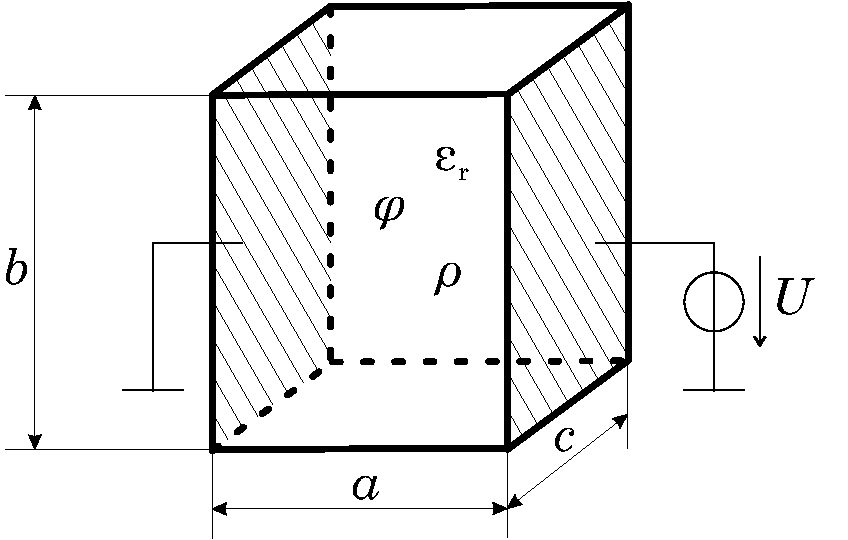
\includegraphics[width=0.6\textwidth]{fig/capacitor.pdf}
\end{center}
\caption{Simple model of a Capacitor in 3D.}
\label{fig:capacitor}
\end{figure}

For example Fig~\ref{fig:simpledyn}. is included using the following commands:
\begin{verbatim}
\begin{figure}[htbp]
\begin{center}
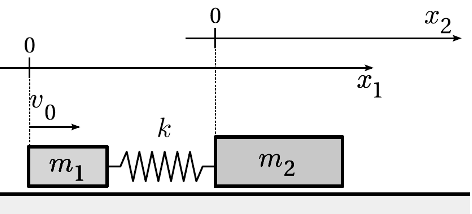
\includegraphics[width=0.6\textwidth]{fig/slbp-bodies.png}
\end{center}
\caption{Simple dynamical system.}
\label{fig:simpledyn}
\end{figure}
\end{verbatim}

\begin{figure}[htbp]
\begin{center}
  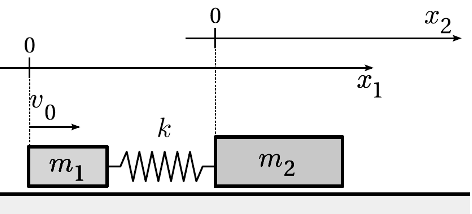
\includegraphics[width=0.6\textwidth]{fig/slbp-bodies.png}
\end{center}
\caption{Simple dynamical system.}
\label{fig:simpledyn}
\end{figure}


\subsection{Tables}

Use standard \verb+tabular+ environment for tables. If possible, avoid
publishing multipage tables in Acta Technica Jaurinensis, try to reorganize
them to smaller tables if possible. If not, use \verb+supertabular+ environment.

Similarly to figures, all tables must be put in \verb+table+ environment
with \verb+\caption+, \verb+\label+ and centering.

The table should be centred, and the relevant caption should be
placed above the table (see Table~\ref{table:simulation}.).
Do not forget to use table caption style.

\subsubsection{An example}

\begin{table}[htbp]
\centering \caption{Table caption}\label{table:simulation}
\begin{tabular}{| c | c | c | c |} \hline
 \textbf{\emph{Column A}} &\textbf{\emph{Column B}} & \textbf{\emph{Column C}} & \textbf{Column D} \\ \hline
  100 \%  	&	50 		&	2		& \textbf{2.24}	   \\ \hline
  90 \%  	&	38 		&	4		& \textbf{2.05}	   \\ \hline
  80 \%  	&	34 		&	0		& \textbf{1.94}	   \\ \hline
  70 \%  	&	20 		&	2		& \textbf{1.75}	   \\ \hline
\end{tabular}
\end{table}

\noindent After the table and figure caption, \verb+\noindent+ command is used.

\subsection{Equations}

Use the standard \LaTeX\ tools for typesetting equations. Labeling of equations
is neccessary only if you refer the equation in the paper.

\begin{equation}\label{eq:01}
  (x+a)^n=\sum_{k=0}^{n} \binom{n}{b} x^{k} a^{n-k}
\end{equation}

\begin{equation}\label{eq:02}
  x=\frac{-b\pm\sqrt{b^2-4ac}}{2a}
\end{equation}



\subsection{Other formatting rules}

The standard way to emphasize text is \verb+\emph{...}+. Never
use \verb+\textbf{...}+ and \verb+\underline{...}+ in text and use them in
tables and figures with special care.

Please, use '\verb+-+', '\verb+--+' and '\verb+---+' consistently as it is
written is standard \LaTeX\ tutorials.

%--------------------
\section{Submitting the \protect\LaTeX\ paper}

A paper written in \LaTeX\  usually consists of many files: a main \LaTeX-file,
figures, possibly special macro packages (see above). All of them must be
packed into a \verb+zip+ archive for simplicity. The name of this zipped file
must be composed by the first one or two authors' family names, i.e.
\verb+Author1Author2.zip+. Please, do not use spaces and accented letters in the
filenames.

A file, describing the compilation of the paper must be included also. Use
\verb+COMPILE.TXT+ for this file. This must include the commands which produces
PDF from the source file. In the most simple case it is only a
`\verb+pdflatex main.tex+' line, but it can be a 2 or 3 line file if you use
\verb+latex+, \verb+pslatex+, \verb+dvipdf+ and similar standard latex versions.

Please compile and include the PDF version for reference. The technical staff 
will set the volume and page numbers and possibly make minor typographical 
corrections before publishing.

%----------------------------------------------------------------------------

\section*{Acknowledgement}
The publishing of this paper was supported by XY.

%----------------------------------------------------------------------------

\begin{thebibliography}{1}

\bibitem{article_a}
V.~A. Szabó, G.~Dogossy, Recycling of mineral water bottles with chemical
  foaming,  \textit{Acta Technica Jaurinensis} 10~(2) (2017) pp. 157--167.
	\newline doi: \begin{footnotesize}\url{https://doi.org/10.14513/actatechjaur.v10.n2.446}\end{footnotesize}

\bibitem{article_b}
E.~Turfa, G.~Dogossy, F.~Ronkay, Improvement of recycled pet properties by
  reactive extrusion,  \textit{Anyagok Világa} 11~(2) (2013) pp. 50--58, in Hungarian.

\bibitem{book}
M.~Kuczmann, A.~Iványi, The Finite Element Method in Magnetics, 1st Edition,
  Akadémiai Kiadó, Budapest, 2008.
	\newline doi: \begin{footnotesize}\url{https://doi.org//10.13140/2.1.3104.1927}\end{footnotesize}

\bibitem{incollection}
M.~Kuczmann, Identification of isotropic and anisotropic vector preisach model,
  in: A.~Iványi (Ed.), Preisach Memorial Book: Hysteresis models in
  mathematics, physics and engineering, 1st Edition, Akadémiai Kiadó,
  Budapest, 2005, pp. 89--102.

\bibitem{conference}
A.~Kovács, G.~Lencse, Modelling of virtualized servers, in: N.~Herencsár,
  K.~Molnár (Eds.), 38th International Conference on Telecommunications and
  Signal Processing: TSP 2015, Brno University of Technology, Brno, 2015, pp.
  241--245.
	\newline doi: \begin{footnotesize}\url{https://doi.org/10.1109/TSP.2015.7296260}\end{footnotesize}

\bibitem{phdthesis}
V.~Nagy, Examination and modeling of porosity in polyester twisted fibrous
  structures, Ph.D. thesis, Budapest University of Technology and Economics
  (2006).
	\newline URL \begin{footnotesize}\url{http://hdl.handle.net/10890/467}\end{footnotesize}

\bibitem{standard}
Plastics -- determination of tensile properties -- part 1: General principles,
  {ISO 527-1:2012} (2012).

\bibitem{patent}
M.~Horski, Brushless motor with inside mounted single bearing, {US 5654598 A}
  (1997).

\bibitem{online}
CostumPartNet,
  \href{http://www.custompartnet.com/wu/InjectionMolding}{Injection molding}
  [cited 2018-01-24].
\newline URL \begin{footnotesize}\url{http://www.custompartnet.com/wu/InjectionMolding}\end{footnotesize}

\bibitem{article_c}
L.~Lendvai, I.~Sajó, J.~Karger-Kocsis, Effect of Storage Time on the Structure and Mechanical Properties of Starch/Bentonite Nanocomposites,  \textit{Starch-Starke} 71~(1-2) (2019) 1800123.
\newline doi: \begin{footnotesize}\url{https://doi.org/10.1002/star.201800123}\end{footnotesize}
	
	\bibitem{article_d}
M.~Gáspár, Z.~Benkő et al., Reducing water absorption in compostable starch-based plastics, 
 \textit{Polymer Degradation and Stability} 90~(3) (2005) pp. 563--569.
\newline doi: \begin{footnotesize}\url{https://doi.org/10.1016/j.polymdegradstab.2005.03.012}\end{footnotesize}

\end{thebibliography}

\begin{table}[ht]
\begin{minipage}{.15\textwidth}
    \begin{tabular}{*{1}{p{0.15\textwidth}}}
\includegraphics[height=5.5mm]{\cc}
\\
\end{tabular}
\end{minipage}% 
\begin{minipage}{.9\textwidth}
    \begin{tabular}{*{1}{p{0.9\textwidth}}}
\footnotesize 
This article is an open access article distributed under the terms and conditions of the Creative Commons Attribution NonCommercial (\href{https://creativecommons.org/licenses/by-nc/4.0/}{CC BY-NC 4.0}) license. \\
\end{tabular}
\end{minipage}%
\end{table}
\end{document}